\subsubsection{Main Use Case Sequence Diagrams}
\label{sec:use-cases-sequence-diagrams}

While a class diagram shows the status structure, sequence diagrams illustrate the dynamic behaviour of the system over time. To demonstrate how the backend orchestrates the logical layers to fulfill user requests, this section presents the sequence of interactions for the two most critical use cases.

Before delving into the sequence diagrams, it is important to note that all API Controllers are protected using the ASP.NET Core authorization middleware through the \texttt{[Authorize]} attribute. This middleware enforces authentication before any request reaches a controller action.

Specifically, before a request reaches the controller, the middleware validates the Azure AD Bearer token included in the request. If the token is invalid or missing, the middleware immediately returns a \texttt{401 Unauthorized} response. If validation succeeds, the user's claims are extracted and made available through the \texttt{CurrentUserService}, and the request is forwarded to the corresponding controller action.


\textbf{Use Case 1: Uploading a New Expense}

This use case showcases the system's hybrid processing model. The initial file upload request is handled synchronously to return an immediate response to the user, while the high computational cost of AI-driven data extraction is isolated to an asynchronous background process. 

\begin{figure}[H]
    \centering
    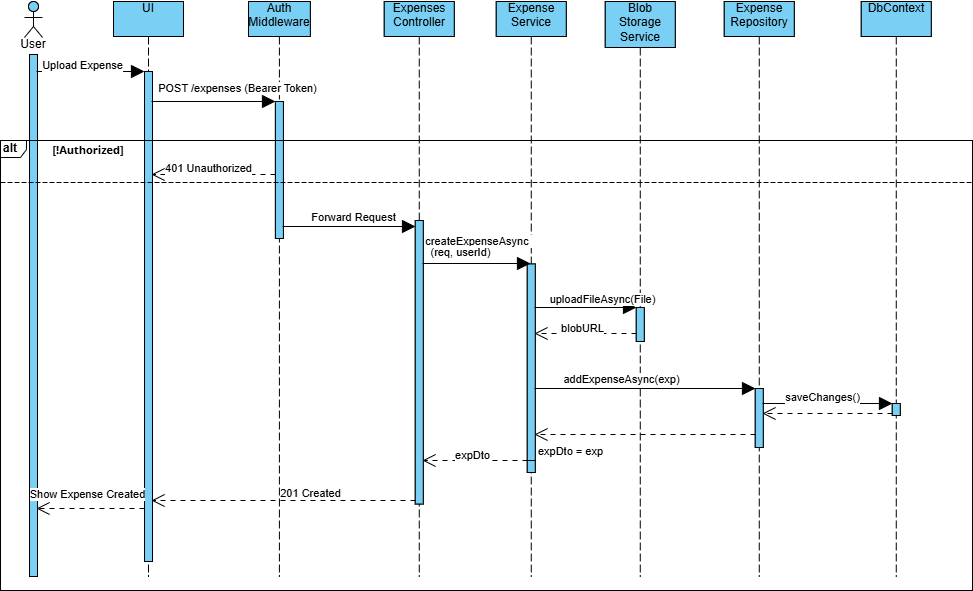
\includegraphics[width=\textwidth]{Images/SeqDiagrams/seq1.png}
    \caption[Sequence diagram for the synchronous Expense upload workflow]
    {Sequence diagram for the synchronous Expense upload workflow. [Own creation]}
    \label{fig:expense-synchronous-sequence-diagram}
\end{figure}

\begin{figure}[H]
    \centering
    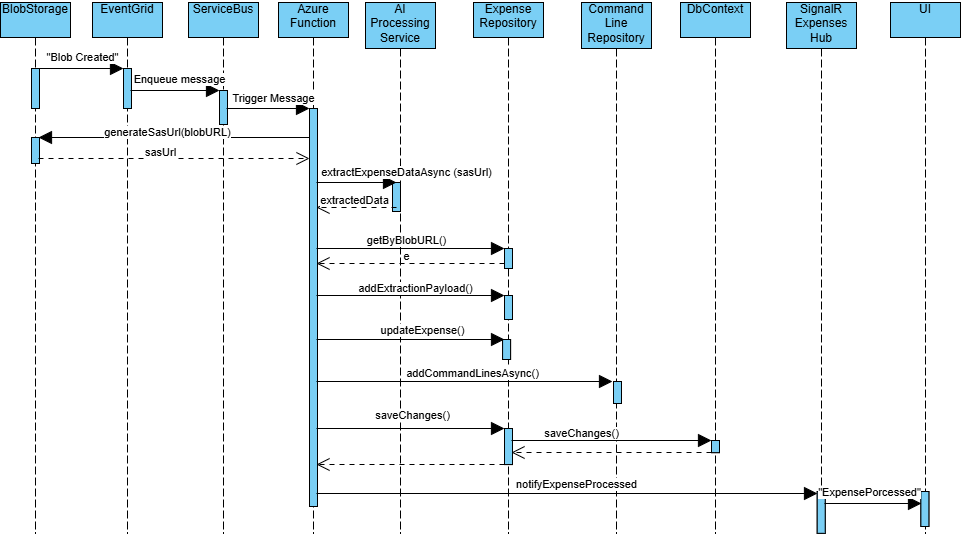
\includegraphics[width=\textwidth]{Images/SeqDiagrams/seq2.png}
    \caption[Sequence diagram for the asynchronous Expense processing workflow]
    {Sequence diagram for the asynchronous Expense processing workflow. [Own creation]}
    \label{fig:expense-asynchronous-sequence-diagram}
\end{figure}

\textbf{Synchronous Expense Upload Process}

Figure \ref{fig:expense-synchronous-sequence-diagram} provides a comprehensive visualization of the synchronous expense upload process. When the user uploads a receipt, the client (UI) sends an HTTP request to the API. If the user is successfully authenticated, the \texttt{ExpensesController} receives the request and delegates the operation to the \texttt{ExpenseService}, which executes the expense creation business logic.

The \texttt{ExpenseService} first calls the \texttt{BlobStorageService} to upload the expense receipt file to Azure Blob Storage. After the upload is completed, the \texttt{BlobStorageService} returns the generated blob URL. 

With this URL in hand, the \texttt{Expense- Service} creates a new \texttt{Expense} entity and passes it to the \texttt{ExpenseRepository}. The repository is responsible for persisting the entity by interacting with the \texttt{ApplicationDb- Context} through Entity Framework Core (EF Core), which ultimately stores the expense metadata in the SQL database.

Once the expense has been successfully persisted, the controller returns a 201 Created response to the client (UI) while the asynchronous expense-processing pipeline continues independently.

\textbf{Asynchronous Background Processing}

After a new expense file is uploaded to Blob Storage, the asynchronous flow represented in Figure \ref{fig:expense-asynchronous-sequence-diagram} is performed in the background. This asynchronous flow was previously illustrated with software resources in the physical architecture diagram in Section \ref{sec:physical-architecture} and corresponds to the Asynchronous AI Processing Flow explained in the same section.

\vspace{1cm}

\textbf{Use Case 2: Approving a Report}

This second use case shows how the system triggers asynchronous email notifications when a report status changes. This use case is also a hybrid approach composed of a synchronous report approval workflow, as shown in Figure \ref{fig:report-approval-sequence-diagram}, which triggers the subsequent asynchronous email notification and publishing flow depicted in Figure \ref{fig:report-publishing-sequence-diagram}.


\begin{figure}[H]
    \centering
    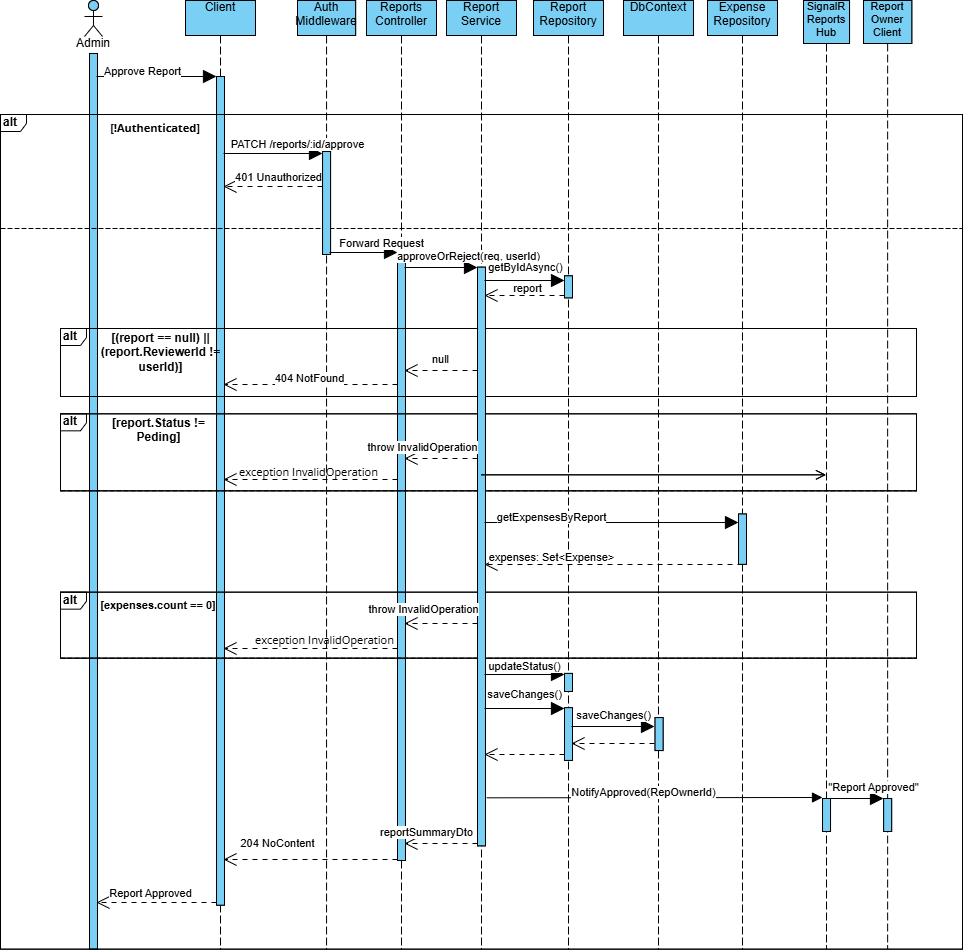
\includegraphics[width=\textwidth]{Images/SeqDiagrams/seq3.png}
    \caption[Sequence diagram for the synchronous Report approval workflow]
    {Sequence diagram for the synchronous Report approval workflow. [Own creation]}
    \label{fig:report-approval-sequence-diagram}
\end{figure}

\begin{figure}[H]
    \centering
    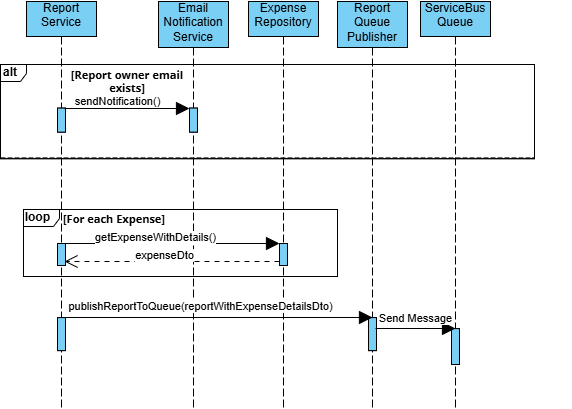
\includegraphics[width=0.6\textwidth]{Images/SeqDiagrams/seq4.png}
    \caption[Sequence diagram for the asynchronous workflow after Report approval]
    {Sequence diagram for the asynchronous workflow after Report approval. [Own creation]}
    \label{fig:report-publishing-sequence-diagram}
\end{figure}

\textbf{Report Approval Workflow}

When an admin user approves a report submitted by an employee under their supervision, the client (UI) sends an HTTP request to the API. After the user is successfully authenticated and the \texttt{ReportsController} receives the request, the operation is delegated to the \texttt{ReportService}, which is responsible for applying the business rules.

The \texttt{ReportService} first verifies that the report exists and that the assigned reviewer matches the authenticated user. If either validation fails, the service returns null to the \texttt{ReportsController}, which subsequently returns a 404 Not Found response to the client.

Next, the \texttt{ReportService} validates that the report status is Pending and that at least one expense is attached to the report. If any of these conditions are not met, an \texttt{InvalidOperationException} is thrown and propagated to the controller, which returns the corresponding error response to the client (UI).

If all business rules are satisfied, the \texttt{ReportService} requests the \texttt{ReportRepository} to update the report status to Approved and persist the changes. The \texttt{ReportRepository} interacts with the \texttt{ApplicationDbContext} through Entity Framework Core (EF Core), which ultimately updates the report record in the SQL database.

Once the report has been successfully approved, the \texttt{ReportService} sends a message through the SignalR \texttt{ReportsHub} to notify the report owner. Finally, the controller returns a \texttt{204 No Content} response to the client (UI), indicating that the operation completed successfully.

\textbf{Email Notification and Publishing after Approval}

Once a report has been approved, the \texttt{ReportService} also performs several background tasks. First, it verifies that the report owner's email address exists to send an email notification informing them that their report has been approved.

\vspace{2cm}

Next, the service retrieves the detailed information for all expenses associated with the report and composes a complete \texttt{ReportWithExpenseDetailsDto}. This DTO is then published through the \texttt{ReportQueuePublisher}, which sends the message to an external service bus queue. The purpose of this final step is to provide data for training an internal AI model.
